\documentclass{beamer}
\usepackage{amsmath,amsbsy,amsopn,amstext,amsfonts,amssymb}
\usepackage{isomath}
\usepackage{ulem}
%\linespread{1.6}  % double spaces lines
\usepackage{graphicx}
\usepackage{subfigure}
\usepackage{color}
\usepackage{optidef}  % define optimization problems
\usepackage{multicol}  % multiple columns
\usepackage{listings} % for python code
\usepackage{mathrsfs}

\usepackage{polynom}
\newcommand{\adj}{\mathrm{adj}}
\newcommand{\constrainedmin}[3]{
		\begin{mini*}|s|
		{#2}{#1}{}{}
		\addConstraint{#3}
		\end{mini*}
}

\newcommand{\rwbcomment}[1]{{\color{blue}RWB:#1}}
\newcommand{\defeq}{\stackrel{\triangle}{=}}
\newcommand{\abs}[1]{\left|#1\right|}
\newcommand{\norm}[1]{\left\|#1\right\|}
\newcommand{\iprod}[1]{\left<#1\right>}
\newcommand{\ellbf}{\boldsymbol{\ell}}
\newcommand{\nubf}{\boldsymbol{\nu}}
\newcommand{\mubf}{\boldsymbol{\mu}}
\newcommand{\abf}{\mathbf{a}}
\newcommand{\bbf}{\mathbf{b}}
\newcommand{\cbf}{\mathbf{c}}
\newcommand{\dbf}{\mathbf{d}}
\newcommand{\ebf}{\mathbf{e}}
\newcommand{\fbf}{\mathbf{f}}
\newcommand{\gbf}{\mathbf{g}}
\newcommand{\hbf}{\mathbf{h}}
\newcommand{\ibf}{\mathbf{i}}
\newcommand{\jbf}{\mathbf{j}}
\newcommand{\kbf}{\mathbf{k}}
\newcommand{\lbf}{\mathbf{l}}
\newcommand{\mbf}{\mathbf{m}}
\newcommand{\nbf}{\mathbf{n}}
\newcommand{\obf}{\mathbf{o}}
\newcommand{\pbf}{\mathbf{p}}
\newcommand{\qbf}{\mathbf{q}}
\newcommand{\rbf}{\mathbf{r}}
\newcommand{\sbf}{\mathbf{s}}
\newcommand{\tbf}{\mathbf{t}}
\newcommand{\ubf}{\mathbf{u}}
\newcommand{\vbf}{\mathbf{v}}
\newcommand{\wbf}{\mathbf{w}}
\newcommand{\xbf}{\mathbf{x}}
\newcommand{\ybf}{\mathbf{y}}
\newcommand{\zbf}{\mathbf{z}}
\newcommand{\Jbf}{\mathbf{J}}
\newcommand{\Acal}{\mathcal{A}}
\newcommand{\Bcal}{\mathcal{B}}
\newcommand{\Lcal}{\mathcal{L}}
\newcommand{\Ncal}{\mathcal{N}}
\newcommand{\Rcal}{\mathcal{R}}
\definecolor{darkolivegreen}{rgb}{0.33, 0.42, 0.18}

\makeatletter
\newenvironment<>{proofstart}[1][\proofname]{%
    \par
    \def\insertproofname{#1\@addpunct{.}}%
    \usebeamertemplate{proof begin}#2}
  {\usebeamertemplate{proof end}}
\newenvironment<>{proofcont}{%
  \setbeamertemplate{proof begin}{\begin{block}{}}
    \par
    \usebeamertemplate{proof begin}}
  {\usebeamertemplate{proof end}}
\newenvironment<>{proofend}{%
    \par
    \pushQED{\qed}
    \setbeamertemplate{proof begin}{\begin{block}{}}
    \usebeamertemplate{proof begin}}
  {\popQED\usebeamertemplate{proof end}}
\makeatother

\title{ECEn 671: Mathematics of Signals and Systems}
\author{Randal W. Beard}
\institute{Brigham Young University}
\date{\today}

\begin{document}

%-------------------------------
\begin{frame}
	\titlepage
\end{frame}



%%%%%%%%%%%%%%%%%%%%%%%%%%%%%%%%%%%%%%%%%%%%%%%%%%%%%%%%%%%%%%%%%
\section{Invariant Subspaces}
\frame{\sectionpage}

%----------------------------------
\begin{frame}\frametitle{Invariant Subspaces}
	\begin{definition}
		Let $A$ be a square matrix.  
		If $\mathbb{S} \subset \mathcal{R}(A)$ is such that $x \in \mathbb{S} \implies Ax \in \mathbb{S}$ then $\mathbb{S}$ is an \underline{invariant subspace} of $A$.
	\end{definition}
	
	\begin{example}
		An eigenvector forms an invariant subspace i.e. 
		\[
			\mathbb{S} = \{\alpha x \mid x \text{~is an eigenvector}\}
		\]
		is invariant since $\hat{x} \in \mathbb{S} \Rightarrow A\hat{x} = \lambda\hat{x} \in \mathbb{S}$.		
		\end{example}
\end{frame}

%----------------------------------
\begin{frame}\frametitle{Invariant Subspaces}
	\begin{example}
		The span of any subset of eigenvectors is invariant:  Let $x_1 \ldots x_p$ be eigenvectors with associated eigenvalues $\lambda_1 \ldots \lambda_p$.
		
		Let 
		\[
			\mathbb{S} = \text{span}\{x_1 \ldots x_p\}
		\]
		then
		\begin{align*}
			& \hat{x} \in \mathbb{S} \\
			\implies & \hat{x} = \alpha_1 x_1 + \cdots + \alpha_p x_p \\
			\implies & A\hat{x} = \alpha_1Ax_1 + \cdots + \alpha_pAx_p \\
			\implies & A\hat{x} = \alpha_1\lambda_1x_1 + \cdots + \lambda_p\alpha_px_p \\
			\implies & A\hat{x} \in \mathbb{S}.		
		\end{align*}
	\end{example}
\end{frame}

%----------------------------------
\begin{frame}\frametitle{Applications to Differential Equations}
	Consider the differential equation 
	\(
		\dot{x} = Ax
	\)
	with initial condition $x(0)=x_0$.
	\begin{lemma}
	 	The solution is given by
	 	\(
	 		x(t) = e^{At}x_0
	 	\)
	 	where $e^{At} = I + At + \frac{1}{2!}A^2t^2 + \frac{1}{3!}A^3t^3 + \cdots$.
	\end{lemma}
	\begin{proof}
		{\footnotesize
		Plug into equation
		\begin{align*}
			\frac{dx(t)}{dt} 
				&= \frac{d}{dt}(e^{At})x_0 + e^{At}\frac{d}{dt}(x_0) 
				= \frac{d}{dt}e^{At}x_0\\
				&= \frac{d}{dt}(I + At + \frac{A^2t^2}{2!} + \frac{A^3t^3}{3!} + \frac{A^4t^4}{4!} + \cdots x_0\\
				&= (A + A^2t + \frac{A^3t^2}{2!} + \frac{A^4t^3}{3!} + \cdots)x_0\\
				&= A(I + At + \frac{A^2t^2}{2!} + \frac{A^3t^3}{3!} + \cdots)x_0\\
				&= Ae^{At}x_0
				= Ax(t)
		\end{align*}
		so $x(t) = e^{At}x_0$ satisfies $\dot{x} = Ax$ with initial condition $x_0$.
		}
	\end{proof}
\end{frame}

%----------------------------------
\begin{frame}\frametitle{Applications to Differential Equations}
	\begin{lemma}
		If $\mathbb{S}$ is an invariant subspace of $A$ then $\mathbb{S}$ is an invariant subspace of $e^{At}$
	\end{lemma}
	\begin{proof}
		Let $x_0 \in \mathbb{S}$ then
		\begin{align*}
			Ax_0 \in \mathbb{S} 
				&\implies tAx_0 \in \mathbb{S} \\
				&\implies A(Ax_0) \in \mathbb{S} \\
				&\implies \frac{A^2t^2}{2!}x_0 \in \mathbb{S} \\
				&\ldots
		\end{align*}
		Therefore
		\[
			x(t) = Ix_0 + Atx_0 + \frac{A^2t^2}{2!}x_0 + \frac{A^3t^3}{3!}x_0 + \cdots \in \mathbb{S}.
		\]
	\end{proof}
\end{frame}

%----------------------------------
\begin{frame}\frametitle{Applications to Differential Equations: Example}
	Consider the differential equation
	\[
		\dot{x} 
			= \begin{pmatrix}
	    		0 & 1\\
	    		2 & -1
	  		  \end{pmatrix} x.
	\]
	The eigenvalues of $A$ are given by
	\(
		\text{det}(\lambda I - \begin{pmatrix}
	    							0 & 1\\
	    							2 & -1
	  							\end{pmatrix}) 
	  	= (\lambda - 1)(\lambda + 2) = 0
	\)
	and so $\lambda_1 = 1$ and $\lambda_2 = -2$.
	
	\vfill
	
	The associated eigenvector are
	\[ 
		x_1 = \begin{pmatrix} 1 \\ 1 \end{pmatrix} 
		\text{ and }
		x_2 =  \begin{pmatrix} 1 \\ -2 \end{pmatrix}.
	\]
\end{frame}

%----------------------------------
\begin{frame}\frametitle{Applications to Differential Equations: Example}
	\begin{center}
		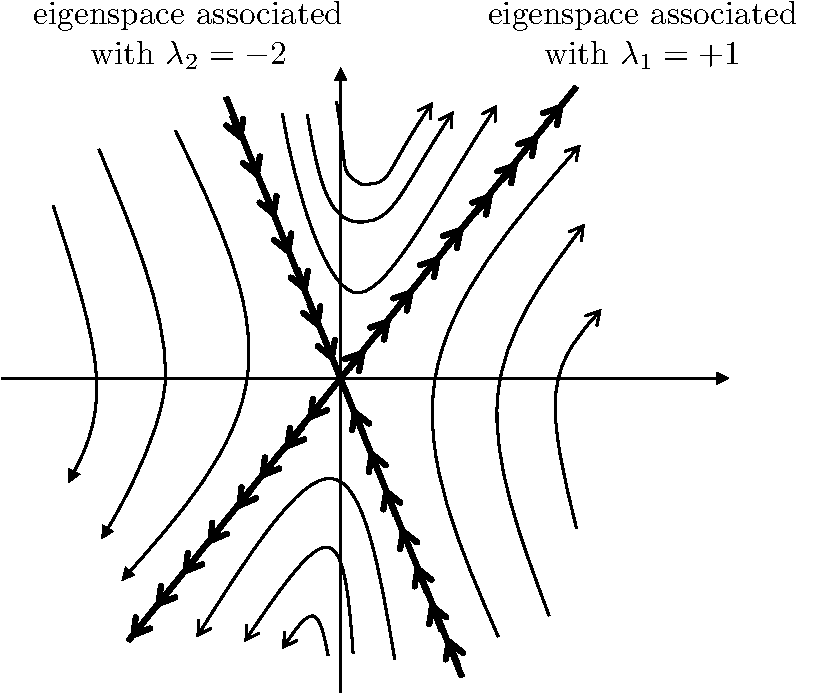
\includegraphics[width=0.7\textwidth]{figures/chap6_invariant_subspaces}
	\end{center}
	
	\begin{itemize}
		\item 	If the initial condition is on $span\{x_1\}$, then the solution remains on $span\{x_1\}$.
		\item If the initial condition is on $span\{x_2\}$, then the solution remains on $span\{x_2\}$.
		\item Otherwise it is a combination of the two modes.
	\end{itemize}
\end{frame}

%----------------------------------
\begin{frame}\frametitle{Applications to Difference Equations: Example}

	\rwbcomment{Change system to eigenvalues in unit circle.  Show that eigenspaces are invariant.  Provide example.}

	Consider the differential equation
	\[
		x[k+1] 
			= \begin{pmatrix}
	    		0 & 1\\
	    		2 & -1
	  		  \end{pmatrix} x[k].
	\]
	Again the eigenvalues of $A$ are $\lambda_1 = 1$ and $\lambda_2 = -2$, and the eigenvectors are
	\[ 
		x_1 = \begin{pmatrix} 1 \\ 1 \end{pmatrix} 
		\quad \text{ and } \quad
		x_2 =  \begin{pmatrix} 1 \\ -2 \end{pmatrix}.
	\]
		
\end{frame}




\end{document}